\documentclass[11pt]{article}
\usepackage{lscape}
\usepackage{graphics}
\usepackage{graphicx}
\usepackage{color}
\usepackage{slashbox}
\usepackage{amsmath}
%\usepackage{times}
\usepackage{overcite}
\usepackage{endnotes}
\usepackage{geometry}
\geometry{letterpaper,tmargin=1in,bmargin=1in,lmargin=1in,rmargin=1in}
\usepackage{setspace}

\setlength{\oddsidemargin}{0cm} \setlength{\evensidemargin}{0cm}
\setlength{\textwidth}{6.5in} %\addtolength{\textheight}{2cm}
\setlength{\textheight}{9in} %\addtolength{\textheight}{2cm}
%\linespread{2}
\renewcommand{\thefootnote}{\fnsymbol{footnote}}

\begin{document}
\title{Peptide identification by tandem mass spectrometry with alternate fragmentation modes}
\author{Adrian Guthals$^{1}$ and Nuno Bandeira$^{1,2,\ast}$}
\date{}
\maketitle

{\centering\small
$^1$ Department of Computer Science and Engineering, $^2$ Skaggs School of Pharmacy and Pharmaceutical Sciences\\
 University of California, San Diego \\
 $^\ast$ Corresponding author: Nuno Bandeira, bandeira@ucsd.edu \\
}
\doublespace

\begin{abstract}
The high-throughput nature of proteomics mass spectrometry is enabled by a productive combination of data acquisition protocols and the computational tools used to interpret the resulting spectra. % \\\ \\
One of the key components in mainstream protocols is the generation of tandem mass (MS/MS) spectra by peptide fragmentation using collision induced dissociation (CID), the approach currently used in the large majority of proteomics experiments to routinely identify hundreds to thousands of proteins from single mass spectrometry runs.
 % \\\ \\ %
Complementary to these, % In addition to CID, %the convenient availability of
alternative peptide fragmentation methods such as electron capture/transfer dissociation (ECD/ETD, respectively) and higher-energy collision dissociation (HCD) have consistently % revealed that these can substantially improve the identification of
achieved significant improvements in the identification of certain classes of peptides, proteins and post-translational modifications.
 % \\\ \\ %
Recognizing these advantages, mass spectrometry instruments now conveniently support fine-tuned methods that automatically alternate between peptide fragmentation modes for either different types of peptides or for acquisition of multiple MS/MS spectra from each peptide.
 % \\\ \\ %
But while these developments have the potential to substantially improve peptide identification, their routine application requires corresponding adjustments to the software tools and procedures used for automated downstream processing.
 % \\\ \\ %
This review discusses the computational implications of alternative and alternate modes of MS/MS peptide fragmentation and addresses some practical aspects of using such protocols for identification of peptides and post-translational modifications.
\end{abstract}

\clearpage

\subsection*{Introduction}

Technological and computational developments continue to expand the fundamental role of tandem mass spectrometry (MS/MS) in high throughput proteomics~\cite{nilsson10}. Current protocols regularly identify thousands of proteins and post-translational modifications (PTMs~\cite{larsen06}) per experiment and can deliver very high levels of reproducibility~\cite{domon10} (e.g. using targeted approaches).
%
%In the large majority of cases, these are enabled by proteolytic digestion of denatured proteins into peptides and rely on peptide identification from Collision-Induced Dissociation (CID) MS/MS spectra using database search tools~\cite{eng11}.
%
%But despite their success, these protocols also tend to "miss / fail to identify" a "wealth" of peptides, proteins and post-translational modifications that are "beginning to be" revealed by emerging alternative MS/MS fragmentation modes.
%
%
%
%But despite their success, the widespread reliance on trypsin digestion of denatured proteins and peptide identification from Collision-Induced Dissociation (CID) MS/MS spectra .
%
%In the large majority of cases, these advances have been enabled by a combination of protocols based on trypsin digestion and Collision-Induced Dissociation (CID) MS/MS spectra
%
%However, these protocols also tend to "miss / fail to identify" a "wealth" of peptides, proteins and post-translational modifications that are "beginning to be" revealed by emerging alternative MS/MS fragmentation modes.
%
%However, these protocols were designed to maximize the number of protein IDs and "fall short" of full coverage, peptidomics, highly-modified peptides, special PTMs.
%
In the large majority of cases, these advances have been enabled by a combination of standard protocols based on trypsin digestion followed by protein identification from collision-induced dissociation (CID) MS/MS spectra using database search tools~\cite{eng11}. The efficiency and reliability of trypsin digestion remains one of the major reasons for the success of high-throughput proteomics. Protein digestion results in multiple peptides per protein and, in the limit, only one peptide needs to be significantly identified to be able to identify the corresponding protein~\cite{gupta09,nesvizhskii10}. Trypsin further contributes to spectrum identifiability in CID MS/MS by cleaving C-term of K/R (Lysine/Arginine) and thus yielding rich and characteristic MS/MS peptide fragmentation patterns~\cite{paizs05,gucinski10} for a substantial subset of all peptides. Incorporating knowledge of these peptide fragmentation patterns into algorithms for MS/MS identification has led to a variety of database search software tools~\cite{eng94,mascot99} for peptide identification by scoring matches between acquired MS/MS spectra and predicted
%\footnote{Some approaches do not explicitly generate predicted MS/MS spectra but rather score peptide-spectrum matches directly using statistical scoring models encoding observed peptide fragmentation patterns~\cite{dancik99,craig04,baker10,kim10cidetd}.}
spectra for peptide sequences extracted from a protein sequence database.

Despite the success of the popular trypsin/CID tandem mass spectrometry protocols, it is well known that this approach generally biases experiments towards the identification of certain types of peptides, such as doubly- and triply-charged peptide precursors from medium-length peptides~\cite{tabb04,zhang04,zhang05,zubarev08,swaney10}. Historically this has been advantageous because CID generates identifiable spectra from these types of peptides (low charge, high m/z) with the greatest efficiency. But a disadvantage of relying upon a single specific protease like trypsin is that many digested peptides are too short and can thus lead to incomplete coverage of the proteome. In the case of trypsin, the enzyme cleaves K/R-rich regions into peptides that are too short for reliable identification (about half of tryptic yeast peptides are $\leq$ 6 residues long~\cite{swaney10}). Alternative protease(s) can be utilized to obtain a wider distribution of peptides and increase coverage. For example, some have demonstrated the value of using of non-specific proteases~\cite{aebersold87,maccoss02a,schlosser05,wang08}, but these can also decrease experimental reproducibility. Another limiting factor is that non-specific proteases can greatly increase the computational search space when matching MS/MS spectra to all possible peptides in the database. This not only increases the time required to search the database, but it can also decrease the sensitivity of spectrum identification at a given false discovery rate (FDR~\cite{nesvizhskii10}). Others have had success using multiple specific proteases (e.g. LysC, AspN, GluC, and ArgC) in a more targeted approach~\cite{swaney10,biringer06,choudhary03}. Compared to the use of a single specific protease, utilizing multiple specific proteases allows for a greater percentage of the proteome (94\% for yeast) to be covered by at least one peptide suitable for mass spectrometry sequencing technology~\cite{swaney10}. If a separate MS/MS run is executed for each enzymatic digestion, there is little increase in computational complexity because MS/MS spectra from each run can be separately matched to a set of peptides cleaved by a single specific protease.

A disadvantage of using multiple proteases is that they often yield peptides that are longer and contain one or more internal basic residues, which are poorly fragmented by CID~\cite{huang05}. But alternative fragmentation strategies such as higher-energy collision dissociation (HCD~\cite{olsen07}, also formerly known as higher-energy C-trap dissociation) and electron transfer dissociation (ETD~\cite{syka04}) are known to improve identification of long, highly-charged peptides, peptides containing basic residues, and peptides containing many or highly-labile PTMs~\cite{coon05,chalkley09,young10,kim12}. A popular strategy has been to use Lys-C in combination with ETD because compared to trypsin, Lys-C generates a larger portion of peptides amenable to efficient ETD fragmentation~\cite{swaney10}. The particular combination of ETD with Lys-N digestion yields peptide coverage complementary to trypsin and very simple fragmentation patterns that can aid in manual de novo peptide sequencing~\cite{taouatas10}. Although the reduction of C-terminal ions in Lys-N ETD peptides reduces the difficulty of manual sequencing, it can also hinder automated approaches that utilize symmetry between N- and C-terminal ions. The complementarity of CID, HCD, and ETD dissociation strategies has been assessed in a variety of contexts~\cite{aguiar10,shen11,jedrychowski11,frese11} and the recognition that each improves identifications of different types of peptides underlies the decision tree~\cite{swaney08,swaney09,swaney10,frese11} approach for real-time selection of fragmentation mode(s) based on each precursor's m/z and charge. Alternatively, CID/ETD~\cite{kim10cidetd} or CID/ETD/HCD~\cite{shen11} alternating MS/MS acquisition for every precursor have also been shown to substantially improve peptide identification and enable otherwise difficult analysis of PTMs~\cite{hogan05}.
%
Underlying the utility of all tandem mass spectrometry approaches to high-throughput proteomics is the need to calculate false discovery rates, usually estimated using the Target/Decoy approach (TDA~\cite{elias07,gupta11}).
%In short, the Target/Decoy Approach (TDA) to FDR calculation consists of adding decoy randomized sequences to the protein sequence database and estimating the expected rate of false positives by ranking all matches by score and using the number of decoy matches with score better than a threshold as proxy for the number of false matches against true sequences. Thus, observing D decoy matches and T matches to the true-sequences (Target) database with scores better than a fixed threshold results in an estimated FDR~\cite{nesvizhskii10} of $\frac{D}{T}$; search results are typically filtered at 1\% FDR.
 %or $\frac{2D}{T+D}$~\cite{elias07}, depending on how the search results are reported.
This approach is a key control of statistical significance in high-throughput proteomics but, as discussed below, requires careful adjustments before it can be meaningfully applied to the analysis of MS/MS data acquired with alternate peptide fragmentation modes.

\subsection*{Peptide fragmentation modes}

While there are several comparisons of peptide fragmentation modes in terms of the resulting numbers of spectrum and peptide identifications, only some~\cite{molina08,zubarev08,chi10,kim10cidetd,hart11} attempt to characterize the observed differences in terms of their underlying MS/MS fragmentation statistics. These matter because the ability of a database search tool to identify MS/MS spectra is proportional to how well it models MS/MS fragmentation statistics and how it uses them to score Peptide Spectrum Matches (PSMs).
%
The basic types of information captured in these peptide fragmentation models are illustrated here using spectra from a recent comparison~\cite{frese11} of how CID, HCD and ETD MS/MS acquisition modes affect Mascot~\cite{mascot99} identifications. In brief, a HeLa tryptic digest was analyzed in three separate Thermo LTQ Orbitrap runs, one for each of CID, HCD and ETD MS/MS acquisition; survey scans were acquired in the Orbitrap with resolution 30000 and MS/MS spectra were acquired in the Orbitrap at resolution 7500. Peptide identifications were obtained here using MS-GFDB as previously described~\cite{kim10cidetd} and resulted in 17,378 CID PSMs (out of 33,586 spectra), 21,246 HCD PSMs (out of 37,810 spectra) and 12,834 ETD PSMs (out of 25,734 spectra). As shown in Table~\ref{tab:ms2ids}, all fragmentation modes achieved comparable spectrum identification rates of $\approx$50\% but also exhibit the expected correlations with precursor charge where ETD tends to perform better than CID or HCD on higher charge states. These show that ETD tends to achieve the highest identification rates for precursors of charge 3 or higher but yet also yields the lowest number of total identifications due to its slower scan rate (only $\approx\frac{2}{3}$ as many MS/MS spectra as in HCD acquisition). Longer acquisition time remains a disadvantage of ETD, however recent work suggests that optimizing ETD acquisition parameters can significantly reduce the scan rate without loss in coverage~\cite{compton12}.
%
The complementarity of the fragmentation modes is further illustrated in Figure~\ref{fig:comp} and supported by the observation that most peptides are not identified by at least one acquisition mode (see supplementary table~\ref{tab:ms2ids-unique}). This is partly due to the different scan rates and the stochastic nature of data-dependent MS/MS precursor selection but, as clearly illustrated for precursor charge 2 (for CID/HCD) and precursor charge 5 (for ETD), this also shows that different peptide fragmentation modes work best for different types of peptides. Of peptides that can be identified by all three acquisition modes, the {\em breaks} (observed cleavages along the peptide backbone, supported by either N- or C-terminal fragments) captured by ETD tend to complement those captured by CID and HCD, especially for precursors of charge 3 or higher. This can be seen in statistics from Figure~\ref{fig:ionstats}, which show how the union of observed peptide breaks increases by 24-72\% from CID/HCD to CID/HCD/ETD for precursors of charge 3 or higher. Supplementary table~\ref{tab:ms2breaks-unique} details how many breaks are unique to every possible combination of fragmentation modes: ETD alone accounts for 19\% of all possible peptide breaks in CID/HCD/ETD triplets, the intersection of breaks seen in CID and HCD accounts for 17\%, and the intersection of breaks seen in CID, HCD, and ETD accounts for 30\%.

The connection between the identifications in Table~\ref{tab:ms2ids} and the underlying MS/MS peptide fragmentation statistics in Figure~\ref{fig:ionstats} is easily established for MS-GFDB PSM scoring models. As previously described~\cite{kim09msdict,kim10cidetd}, MS-GFDB uses the exact same computational model to learn MS/MS fragmentation statistics for CID, HCD and ETD and weigh different MS/MS fragment ion types based on their observed propensity in spectra from each fragmentation mode. The predominant CID, HCD and ETD ion types and their relative propensities are shown in Figure~\ref{fig:ionstats}. As expected, the most prominent differences in peptide fragmentation pertain to the contrast between the dominant $b$/$y$-ions in CID/HCD spectra and $c$/$z$-ions in ETD spectra. These ions are the most important in peptide identification because of their direct indication of peptide breaks; Figure~\ref{fig:ionstats} compares the fractions of observed breaks on peptides identified on all three fragmentation modes. Not surprisingly, the per-precursor-charge fractions of observed breaks on CID, HCD and ETD show a very high correlation with the relative identification rates in Table~\ref{tab:ms2ids} as higher fractions of observed breaks almost always result in higher rates of identified spectra.

The complementarity of different peptide fragmentation modes in yielding identifications for different classes of peptides was the underlying principle behind the Decision Tree (DT) acquisition mode~\cite{swaney08,frese11} where MS/MS acquisition modes are selected in real time based on precursor m/z and charge. Decision tree parameters are usually set to maximize the resulting number of peptide identifications and thus implicitly encode instrument-specific tradeoffs between scan rates and the expected rate of success in post-acquisition spectrum identification. Since the latter is highly dependent on the type of mass spectrometry experiment (e.g., shotgun proteomics~\cite{swaney08} vs phosphoproteomics~\cite{aguiar10,kim11}) and on the success rates of the software tools chosen for spectrum identification, it is important to note that optimal decision tree parameters may vary between instrument models/methods and depend on the choice of software tools used for peptide identification.

% Combination of alternate modes

%De novo
%\begin{itemize}
%    \item ** manual usage of MS3 spectra as an aid to de novo sequencing~\cite{lin98}
%    \item ** MS2/MS3 intersection spectra, scoring by multiplied/summed peak intensity~\cite{zhang00}
%    \item ** De novo sequencing with CID/ECD pairs, non-probabilistic arbitrary scores~\cite{horn00,savitski05a}
%    \item ** MS2/MS3 pairs, statistical scoring~\cite{bandeira08}
%    \item ** CID/ETD pairs, Bayes networks scoring~\cite{datta09}
%    \item ** CID/ETD pairs, non-probabilistic, intensity-based scoring~\cite{bertsch09}
%\end{itemize}

\subsection*{Peptide identification}

The complementarity of multiple peptide fragmentation modes can also be used to improve peptide identification by combining multiple spectra for the same peptides. One of the earliest such approaches was the utilization of MS/MS/MS (MS$^3$) acquisition for de novo peptide sequencing~\cite{lin98}, later automated with heuristic~\cite{zhang00} and optimal~\cite{bandeira08mann} algorithms. Similar applications to de novo peptide sequencing were also introduced at about the same time~\cite{horn00} for paired CID and Electron Capture Dissociation (ECD) spectrum acquisition from the same precursors, also later automated for CID/ECD pairs~\cite{savitski05a} and CID/ETD pairs~\cite{datta09,bertsch09}. In all cases, automated de novo sequencing was improved by combining ions in the MS$^2$/MS$^3$ or in the paired CID/ExD spectra using either combined peak intensities~\cite{zhang00,horn00,savitski05a,bertsch09} or statistical scoring models~\cite{bandeira08mann,datta09}. Current de novo applications of CID/HCD/ETD and MS$^3$ remain heavily dependent on manual interpretation with some assistance from automated methods~\cite{medzihradszky12}.
%
%Database search
%\begin{itemize}
%    \item MS2/MS3 of synthetic peptides used for manual validation of peptide IDs in peptidomics~\cite{kalkum03}
%    \item Probabilistic score used to combined IDs from MS2 and MS3 spectra~\cite{olsen04}
%    \item S-score proposed to assess spectral quality and quality of matches for paired CID/ECD spectra~\cite{savitski05}
%    \item Paired CID/ETD database search: combining results with intersection strategies~\cite{molina08}
%    \item Merged CID/ETD spectra don't work for Mascot phosphopeptide searches~\cite{kim11}
%\end{itemize}
%

Although database search tools developed for CID can be used for HCD and easily adapted to process ETD (by simply examining $c/z^{\circ}$ ion offsets instead of $b/y$), they would likely perform much worse than tools that are sensitive to unique features of HCD and ETD. Features of HCD that are not captured by CID scoring models include peaks in the low $m/z$ range (including immonium ions), high fragment mass resolution (most CID spectra have low fragment mass resolution) and the presence of internal ions. Aside from $c/z^{\circ}$ ions, ETD spectra typically contain charge-reduced precursor peaks with high intensity, characteristic losses from charge-reduced precursors and additional related ions at offsets $\pm H$ from $c$ and $z^{\circ}$ ions. Thus, CID scoring models should be re-designed for HCD and ETD in order to be most effective. The difficulty of the adaptation depends on the algorithm being considered. For example, MS-GFDB~\cite{kim10cidetd} can be automatically re-trained for new types of spectra with only 1,000 PSMs from unique peptides (per precursor charge state). Most CID database search tools~\cite{eng11,eng94,perkins99,craig04,bern07,tabb07,wang07,spivak09} have been extended to support identification of ETD MS/MS spectra: OMSSA~\cite{geer04}, ProteinProspector~\cite{baker10}, MS-GFDB~\cite{kim10cidetd}, PeaksDB~\cite{liu10}, Trans-Proteomic Pipeline~\cite{deutsch10}. However, database search using alternate fragmentation modes remains a less explored approach due to two key issues: $i$) how to best combine multiple spectra from the same precursor and $ii$) how to calculate experiment-wide false discovery rates when CID, HCD and ETD PSM scores may not be directly comparable.

\subsubsection*{Estimation of false discovery rates}

As suggested by the MS/MS fragmentation statistics in Figure~\ref{fig:ionstats}, database search tools trained to identify CID spectra will not perform well if given ETD or CID/ETD merged peak lists~\cite{kim11}. A more careful combination of CID/ECD MS/MS spectra for de novo sequencing was first described over a decade ago~\cite{horn00,savitski05a} and later approaches~\cite{datta09,kim10cidetd} have extended their statistical scoring models to incorporate CID- and ETD-specific ions into merged spectra that are then searched appropriately. In these cases PSM scores are directly comparable and standard FDR calculations~\cite{elias07} suffice to reveal substantial gains in peptide identification. An alternative approach to the creation of merged spectra is to separately search the multiple spectra from the same precursors and later merge the search results. This approach simplifies the reutilization of existing database search tools for additional alternate fragmentation modes but complicates the FDR calculations because, for example, a score threshold of 40 may yield a 1\% FDR for CID matches but a 4\% FDR for ETD matches. One possible way to address such discrepancies is to derive statistical e-value models for each type of search~\cite{alves07,alves10} and use the resulting normalized values to combine search results, similarly to approaches devised to combine search results from multiple search tools~\cite{alves08}. To avoid the need for score normalization, intersection-based approaches~\cite{molina08} address this issue by requiring matching identifications from {\em both} CID and ETD spectra to accept an identification for each precursor but unfortunately this is known~\cite{kim10cidetd} to lower the number of resulting identifications by requiring significant matches from both CID and ETD spectra. Union-based approaches are often also mentioned where one imposes a 1\% FDR on separate CID and ETD searches and reports the union of results; unfortunately this approach can result in a combined FDR higher than 1\% because correct identifications will match the same peptide but incorrect identifications mostly accumulate. In practice, a simple strategy for 1\% FDR estimation with $k$ alternate acquisition modes would be to impose an FDR threshold of $1/k$ on each separate search, thus leading to merged results with accumulated false positives at $\leq$~1\%~FDR. However, this is known to be a conservative strategy that is likely to be less sensitive than existing methods for combining search results from different search tools~\cite{alves08,searle08,spivak09,shteynberg11}, which can also be adapted for the identification of spectra from experiments using alternate fragmentation modes, including Decision Tree-based MS/MS acquisition protocols~\cite{swaney08}. Another possible approach to this issue is to combine the search scores prior to FDR calculations. This approach was used in the first extension to multi-spectrum database search by deriving combined Mascot/probability scores for MS$^2$/MS$^3$ spectrum pairs~\cite{olsen04}. These approaches~\cite{ulintz08,kim10cidetd} avoid the intersection/union difficulties by using combined scores to facilitate FDR calculations and allow identifications where one fragmentation mode results in a good spectrum even if the other mode results in a poor spectrum. It is expected that combining search engines for CID, HCD and/or ETD also improves results, but it is important to combine these approaches with appropriate estimation of FDR (such as iProphet~\cite{shteynberg11}).

%\begin{itemize}
%\item CID: (almost everyone) SEQUEST~\cite{eng94}, MASCOT~\cite{perkins99}
%\item ETD: OMSSA \cite{geer04}, X!Tandem \cite{craig04}, Protein Prospector \cite{chalkley05_1, chalkley05_2},
% SEQUEST \cite{eng94}, MASCOT \cite{perkins99}, MyriMatch \cite{tabb07}, pFind \cite{wang07}, Phenyx \cite{colinge03a}, ByOnic \cite{bern07}, ProteinScape \cite{chamrad03}, MS-GFDB \cite{kim10}, SpectrST \cite{lam07}, Peaks DB \cite{liu10}, IDPicker \cite{ma_zd09}, InspecT \cite{tanner05}, Spectrum Mill (Agilent Technologies), MSQuant \cite{mortensen10}, Mascot Distiller \cite{schmelzer04}, Percolater \cite{spivak09}, iProphet \cite{shteynberg11}, ProteoWizard \cite{kessner08}, Trans-Proteomic Pipeline \cite{deutsch10}
%\item HCD: SpectrumMill, MS-GFDB (similar to QTOF - mention those engines?)
%\end{itemize}

% PTMs: ID and localization

\subsubsection*{Post-translational modifications}

Identification of post-translational modifications stands to benefit substantially from MS/MS analysis with alternate fragmentation modes, especially those involving electron-based dissociation modes~\cite{zubarev03,mikesh06}. One of the earlier such approaches~\cite{beausoleil04} is the still popular phosphoproteomics protocol~\cite{palumbo11} where MS$^3$ acquisition is triggered by the dominant loss of phosphate from precursor ions observed in MS$^2$ spectra. Alternating MS/MS modes further improve identification of phosphorylated peptides~\cite{swaney09,kim11,palumbo11} and, in addition, enable otherwise challenging experiments such as co-identification of glycans and peptides from glycosylated peptides using ETD~\cite{chen12} or alternating CID/ETD acquisition~\cite{hogan05,hanisch12}. The complementarity of CID and ETD fragmentation modes is especially useful for PTMs such as glycosylation since CID leads to preferential fragmentation of the more labile glycosidic bonds and generally poor peptide fragmentation, thus facilitating glycan identification but complicating peptide identification. Conversely, ETD fragmentation of glycosylated peptides tends to result in series of $c$- and $z$-ions much like with unmodified peptides and thus facilitates peptide identification and localization of the site of glycosylation.

Accurate localization of PTM sites is also an important area that stands to gain from alternate~\cite{aguiar10,palumbo11,jedrychowski11} and alternative~\cite{nagaraj10} peptide fragmentation modes.
%
As recently reviewed by Chalkley~and~Clauser~\cite{chalkley12}, the problem of PTM site localization was first addressed with the AScore approach~\cite{beausoleil06} which assigns a probabilistic score to a site assignment based on the number of observed ions distinguishing the top-scoring site assignment from the runner-up site assignment. More recent approaches have slightly adapted this concept to assign site assignment scores based on the difference of database search scores between the top and runner-up peptide-spectrum matches to each spectrum from a modified peptide. In all cases, the key factor determining the significance of site assignments is the presence or absence of MS/MS ions in between the possible sites of post-translational modification. Since it is clear from Figure~\ref{fig:ionstats} that alternate fragmentation modes tend to increase observation of peptide breaks, it is expected that the utilization of such modes will result in different numbers and quality of site assignments~\cite{aguiar10,taus2011}, even though strategies for estimation of false-positive site assignments (False Localization Rates~\cite{chalkley12}) are still in their infancy.
%
In addition to improving PTM site localization by increasing the numbers of observed $b$/$y$-ions, one especially interesting feature of HCD MS/MS acquisition is its generation of $x$-ions that are very specific indicators of phosphorylation sites~\cite{kelstrup11}. These are hypothesized to derive from the phosphoric acid being a much better leaving group than water on Serines and Threonines and hence was observed to be a precise indicator of phosphorylation sites, though it was found in only ~33\% of all phoshphorylated peptides.

% Peptidomics?

% Gygi04 Phospho MS3~\cite{beausoleil04}
%Approximately 50% of all MS/MS/MS spectra contained no useful information because there was an insufficient number of ions isolated. This problem resulted in only 96 of 2,002 phosphorylation sites being determined only from an MS/MS/MS spectrum. However, in hundreds of cases, the MS/MS/MS spectra were useful to aid in site localization and in confirming the identification of matching MS/MS spectra. For MS/MS�MS/MS/MS pairs with lower-scoring MS/MS spectra (Xcorr < 2.5), average MS/MS/MS scores were increased by 10%. When the Xcorr for the MS/MS was >2.5, the average MS/MS/MS score showed no improvement.

% Olsen04 Phospho MS3~\cite{olsen04}
%We have expressed the likelihood for random match as �10 � log(P), to make them comparable to the output of the mascot search engine (10). The algorithm used in mascot is not published but also involves probability-based matching. Therefore, the total probability of the MS2 and the MS3 matches to be incorrect should be the product of the probabilities of the mascot and the MS3 score calculated here, and the combined score should be the sum of the scores since they are expressed as logarithms.

%While there are several assumptions and caveats underlying the estimation of FDRs~\cite{nesvizhskii10,gupta11}, one implicit assumption that is especially relevant here is that the scores used to rank peptide spectrum matches should be comparable - that is, a match $m=(s,p)$ of a spectrum $s$ to a peptide $p$ is better than a match $m'=(s',p')$ of a spectrum $s'$ to a peptide $p'$ if $score(m)>score(m')$.

%\subsection{Library search}
%\begin{itemize}
%\item CID: M-SPLIT, BiblioSpec, XHunter, SpectraST
%\item ETD: SpectraST
%\item HCD: pSearch? (from pNovo's group?)
%\end{itemize}

\subsection*{Conclusions and outlook}

%\begin{itemize}
%\item Alternate fragmentation modes substantially increase fraction of identified precursors
%\item Key in some applications where one mode identifies glycans (CID) and the other identifies peptides (ETD) - reference?
%\item FDR issues exist but there are methods available to handle them
%\item More tools and workflows natively support alternate fragmentation mode searches: Sequest, Mascot, MS-GFDB, TPP, Scaffold~\cite{searle08}
%\item Scan rate tradeoff is still high - need to decide whether to go for more peptides or higher identification rate.
%\end{itemize}

The substantial advantages of peptide identification with alternate fragmentation modes have been clearly demonstrated in a variety of contexts~\cite{horn00,hogan05,datta09,chowdhury09,kim10cidetd,shen11,jufvas11,lu11} but their widespread adoption remains limited by two significant hurdles: $i$) the scan rate tradeoff between increasing the chances of identifying each peptide versus just acquiring spectra for more distinct peptides and $ii$) the evolving but limited support of peptide identification tools for taking advantage of alternate fragmentation modes.

The scan rate tradeoff is a challenge that will continue to be addressed with technological developments such as those that brought us the current generation of mass spectrometry instruments, some of which are already able to generate tens of thousands of MS/MS spectra per hour~\cite{duncan10}. Nevertheless, alternate fragmentation has already been shown to be useful in key areas or potential therapeutic relevance~\cite{depontieu09,walsh10,robertson11,king11} such as peptidomics~\cite{shen11} and post-translational modifications analysis such as glycosylation~\cite{hogan05}, phosphorylation identification and site localization~\cite{lu11,aguiar10} and histone modifications~\cite{jufvas11}.

The challenge of limited software support is well on its way to resolving itself as more and more peptide identification tools~\cite{datta09,chi10,baker10,kim10cidetd,deutsch10,liu10} add support for alternative MS/MS fragmentation modes. Still, too few tools support integrated analysis of multiple fragmentation modes~\cite{kim10cidetd}. Although the concept of combining fragmentation modes is over a decade old~\cite{horn00}, most existing scoring functions for peptide identification process CID, HCD, and/or ETD spectra individually. But possibly the biggest hurdle in the development of new software tools is the recurring limited public availability of mass spectrometry data. For example, only 5 out of over 120 published papers on CID/ETD have deposited their raw data~\cite{swaney08,burkard09,kim10cidetd,kim11,savitski11} on Tranche/ProteomeCommons~\cite{falkner07} or PeptideAtlas~\cite{desiere06}. This is a limitation that disproportionably affects the most novel and least common types of mass spectrometry experiments. We hope that the growing trend of making raw data publicly available will catch up with the dominant public availability of software tools and continue the self-reinforcing cycle towards better and more robust peptide identification strategies.

\subsection*{Acknowledgements}
This work was partly supported by the National Institutes of Health grant 1-P41-RR024851 from the National Center for Research Resources.

\clearpage
\singlespace

\begin{figure}[htb!]
\centering
%\vspace{-8 mm}
\hspace{-2 mm}
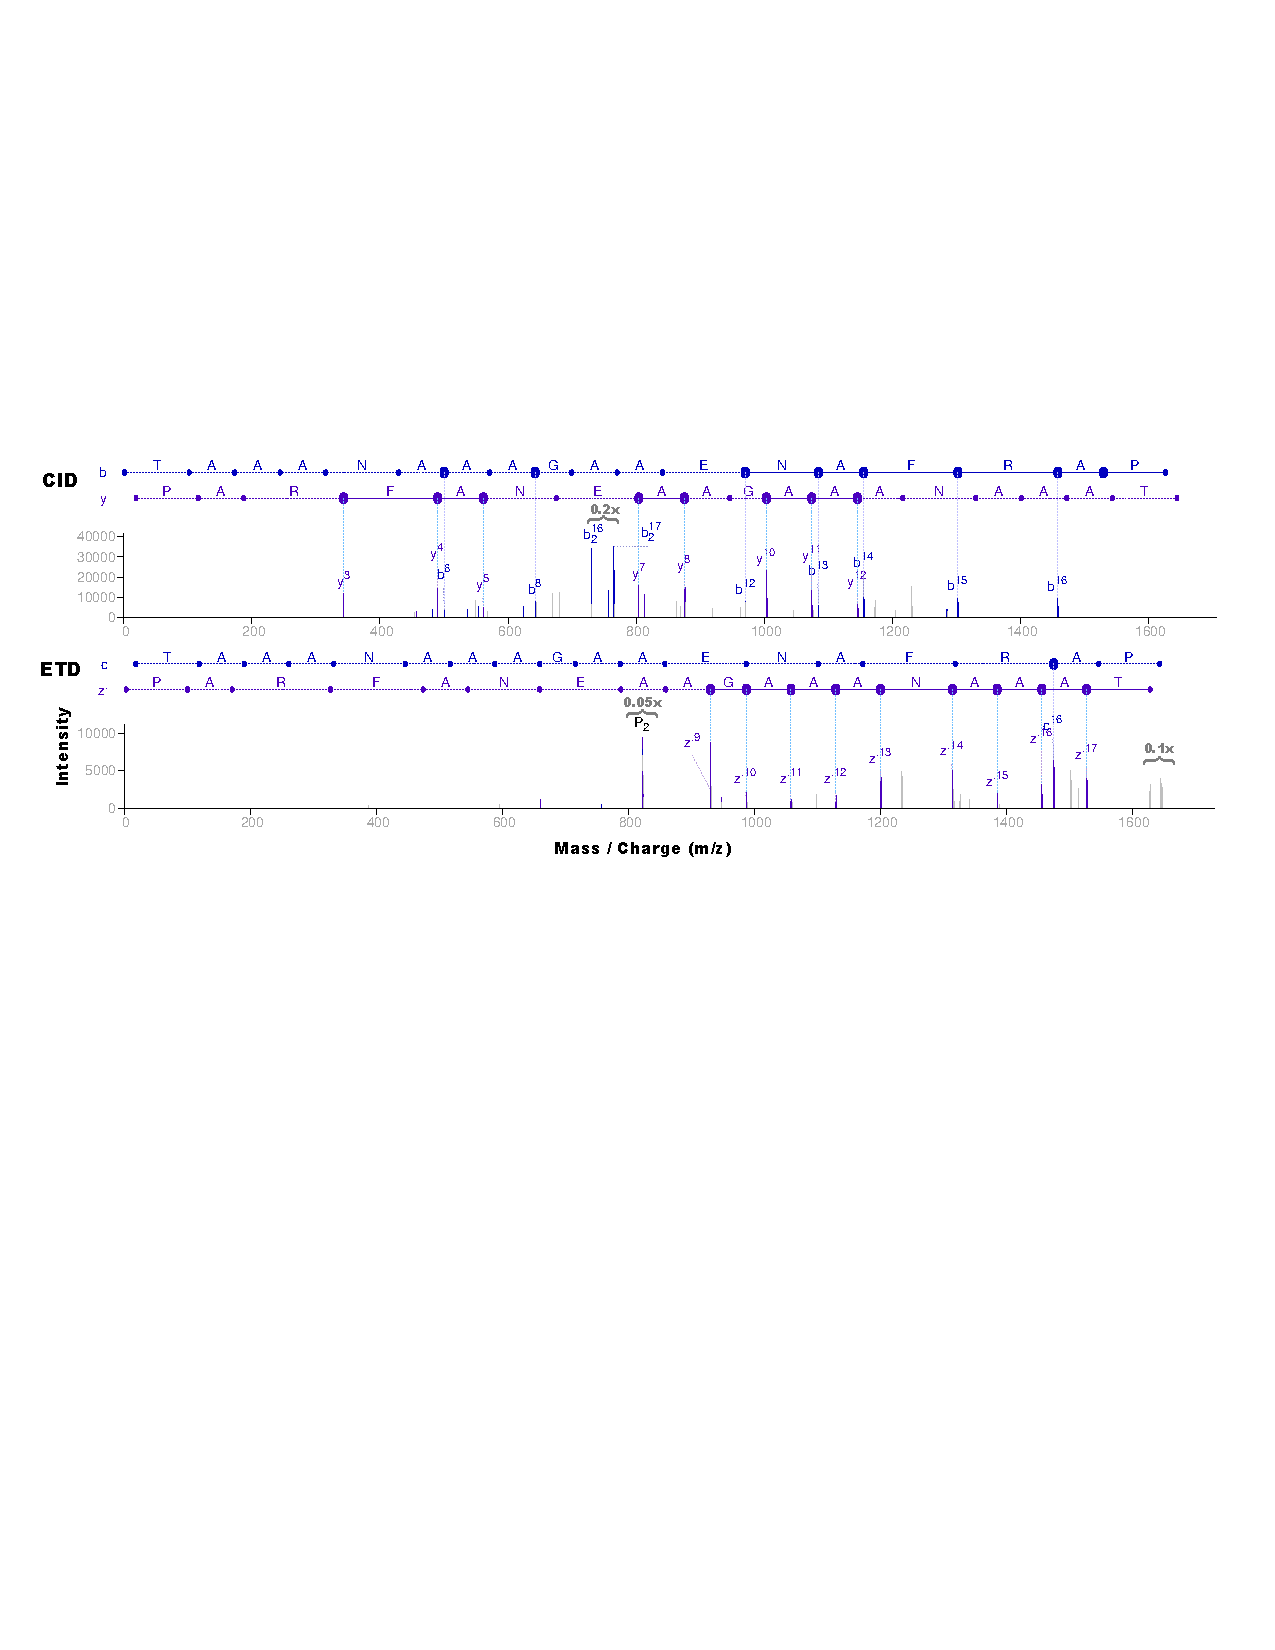
\includegraphics[scale=0.82]{figures/figure1}

\caption{Complementary fragmentation in CID and ETD for peptide TAAANAAAGAAENAFRAP. CID (top) and ETD (bottom) spectra were separately identified against this C-terminal tryptic peptide at 1\% FDR. Enough ions were separately detected in each spectrum to identify the peptide (65\% of breaks in CID, 53\% in ETD). But combining the two yields full coverage of all possible breaks, thus giving higher confidence to breaks observed in both spectra and possibly enabling full-length de novo sequencing. See Figure~\ref{fig:ionstats} and supplementary table~\ref{tab:ms2breaks-unique} for evidence of CID/ETD complementarity over all identified spectra.}
\label{fig:comp}
\end{figure}

\clearpage

%\footnotesize
\begin{table}[htb!]
%\small
%\footnotesize
\centering
\begin{tabular}{lcccccccc}
%    & \multicolumn{3}{c}{N-term ions} & & \multicolumn{2}{c}{C-term ions} \\
%\cline{2-4}
%\cline{6-7}
& \multicolumn{2}{c}{CID} & & \multicolumn{2}{c}{HCD} & & \multicolumn{2}{c}{ETD}\\
\cline{2-3}
\cline{5-6}
\cline{8-9}
All Charges & 17378 & 51.7\% && 21246 & 56.2\% && 12834 & 49.9\%\\
Charge 2 & 10031 & 56.0\% && 11880 & 59.4\% && 6058 & 44.1\%\\
Charge 3 & 5719 & 49.2\% && 7485 & 56.7\% && 5076 & 57.0\%\\
Charge 4 & 1408 & 43.6\% && 1644 & 44.9\% && 1391 & 56.8\%\\
Charge 5 & 206 & 29.3\% && 213 & 26.6\% && 262 & 47.5\%\\
Charge 6 & 13 & 12.9\% && 23 & 20.2\% && 42 & 51.9\%\\
%Charge 7 & 1 & 6.2\% && 1 & 3.8\% && 5 & 50.0\%\\
\end{tabular}\\
%\flushleft
%\scriptsize
\caption{Identified Peptide-Spectrum Matches (PSMs) for alternative fragmentation modes. Each column shows the number of identified PSMs and the corresponding fraction of identified spectra per precursor charge state. As expected, the identification rate for ETD spectra is higher for precursors with charge states 3 or higher, in contrast with CID/HCD which tend to perform best for doubly-charged precursors. Nevertheless, the currently slower ETD scan rate (an issue that may be resolved soon~\cite{compton12}) still leads to lower numbers of identified spectra with precursor charges 3 and 4 even though its identification rate is consistently higher than those of CID and HCD spectra; this tradeoff seems to disappear at precursor charge states 5 and higher, where ETD consistently identified more spectra and a higher percentage of precursors than either CID or ETD.}
 \label{tab:ms2ids}
\end{table}
%\normalsize

\begin{figure}[htb!]
\begin{minipage}[c][60mm]{0.40\linewidth}
%\centering
%\vspace{8 mm}
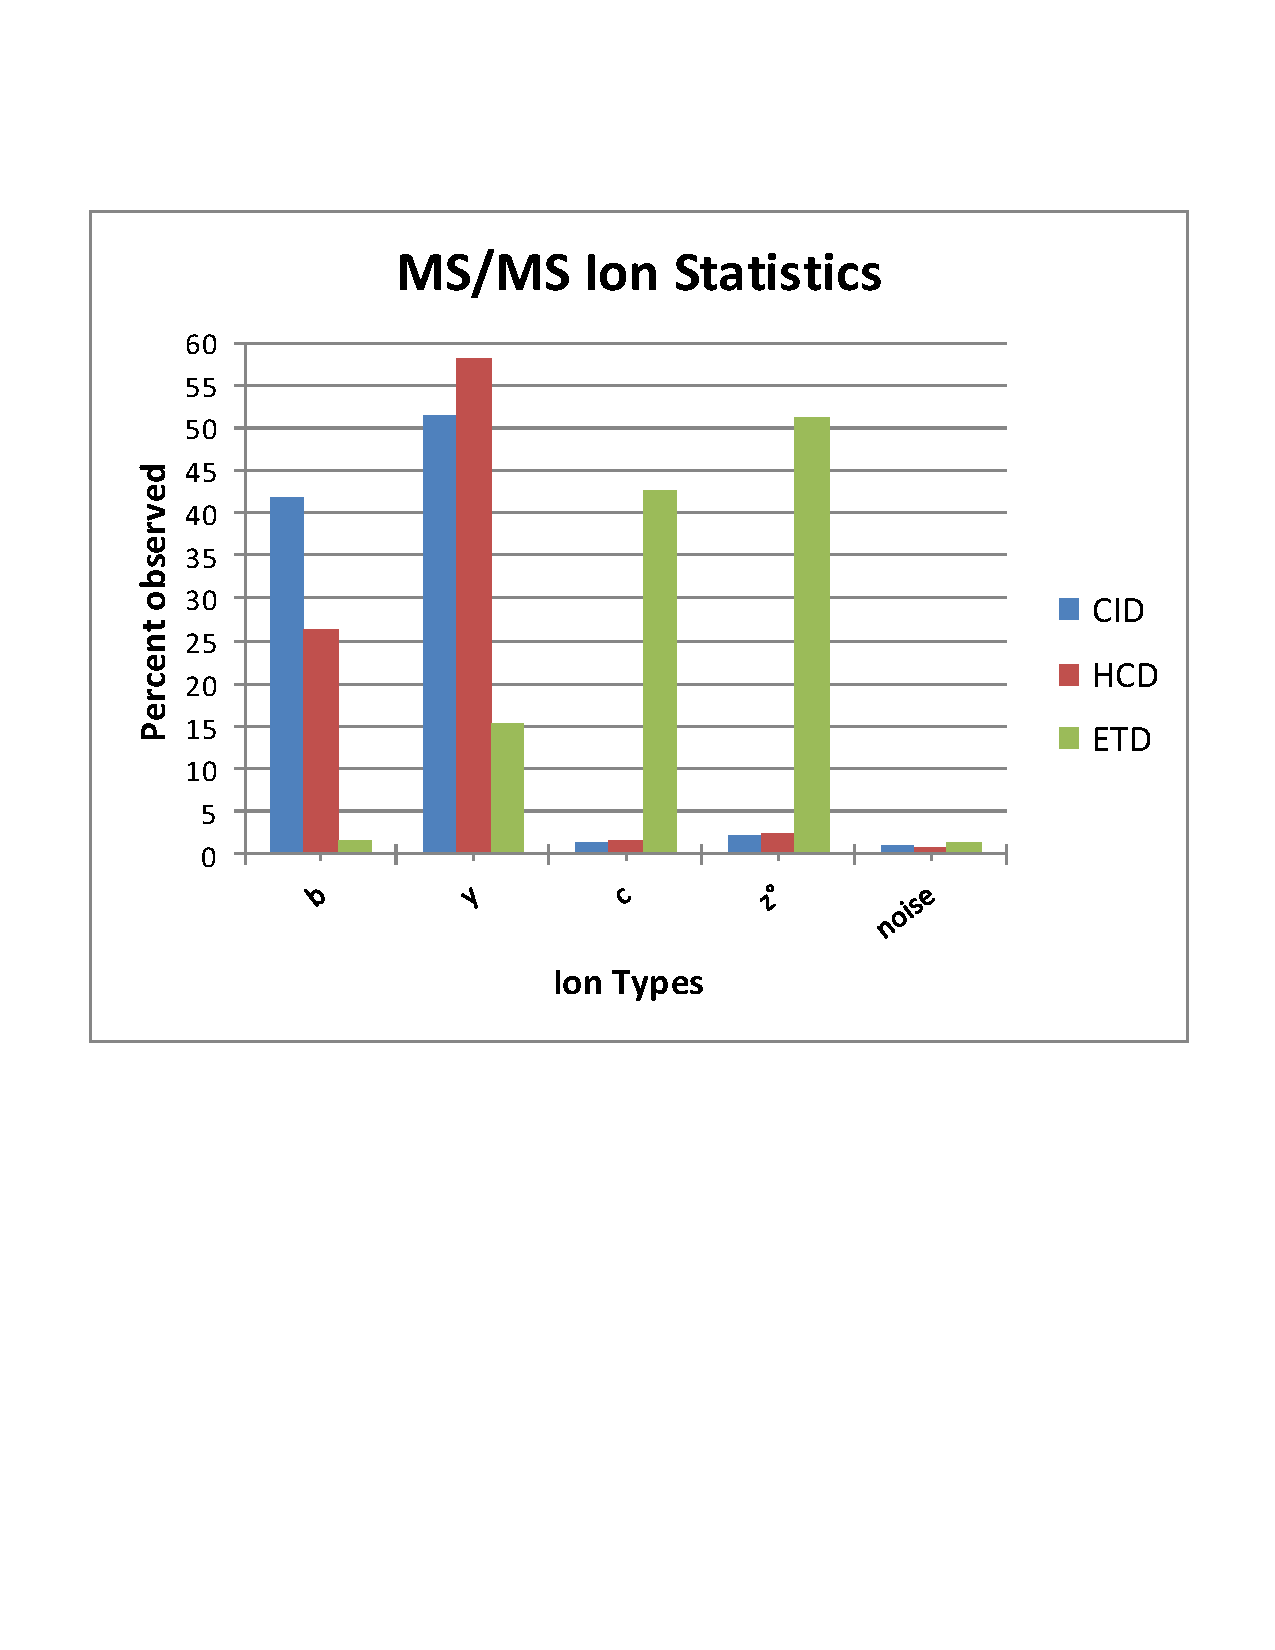
\includegraphics[scale=0.35]{figures/Heck_ion_stats}
\end{minipage}
\begin{minipage}[c][60mm]{0.60\linewidth}
%\centering
%\vspace{45 mm}
\begin{tabular}{rccccc}
    & \multicolumn{5}{c}{Peptide Breaks}\\
\cline{2-6}
Prec. Charge  & $2$ & $3$ & $4$ & $5$ & All \\
\# Unique Pep. & 4361 & 2873 & 712 & 87 & 8037 \\
CID & 72.3 & 45.7 & 32.2 & 25.7 & 55.8\\
HCD & 74.1 & 54.0 & 34.9 & 27.1 & 60.3\\
ETD & 64.1 & 63.6 & 55.9 & 40.4 & 62.4\\
CID/HCD & 83.9 & 61.9 & 42.5 & 33.4 & 69.0\\
CID/ETD & 88.9 & 80.7 & 70.7 & 56.5 & 82.8\\
HCD/ETD & 89.1 & 84.3 & 72.1 & 57.4 & 84.4\\
CID/HCD/ETD & 93.2 & 86.8 & 75.4 & 61.1 & 87.8\\
\end{tabular}
\end{minipage}
\caption{Ion statistics for alternative peptide fragmentation modes. \textbf{(Left)} Peptide MS/MS ion statistics for alternative fragmentation modes - This shows the percentage of breaks observed by each ion type over all identified MS/MS spectra with precursor charge 2 or 3 for each fragmentation method. $z ^{\circ}$ corresponds to peaks at offset +H from $z$ ions \cite{savitskim07}. Ions were counted if observed peak masses were within 20 ppm of expected ion masses. The "noise" ion corresponded to offset $b+0.5$, which was counted to show the level of noise in each type of MS/MS spectra. \textbf{(Right)} Peptide break statistics for combinations of alternative fragmentation modes - peptide breaks were counted for all unique peptides identified by all three fragmentation modes. The 6 columns show the percentage of breaks detected by each fragmentation mode and combination of fragmentation modes per precursor charge state. In CID and HCD spectra, the presence of breaks were indicated by the presence of $b$ or $y$ ions. For ETD, $c$, $z ^{\circ}$, or $z ^{\circ} \medspace + \medspace $H ions indicated the presence of a break. Multiply charged ions (up to the spectrum's precursor charge) were also considered in each spectrum. Prior to this analysis, peak filtering was applied all CID, HCD, and ETD spectra such that each peak was retained only if its intensity was ranked 5th or higher over all neighboring peaks in a +/- 56 Da radius. If a peptide was identified by more than one CID, HCD, or ETD spectrum, a single representative spectrum was randomly chosen for each fragmentation mode.}
\label{fig:ionstats}
\end{figure}

\clearpage




\bibliographystyle{unsrt}
%\bibliographystyle{plain}
%\bibliographystyle{alpha}
\bibliography{../bibtex/msms,../bibtex/bandeiraLab}

\clearpage

%\appendix
%\renewcommand\thesection{Appendix~\Alph{section}}
\renewcommand{\thefigure}{SM-\arabic{figure}}  % redefine the command that creates the equation no.
\setcounter{figure}{0}  % reset counter
\renewcommand{\thetable}{SM-\arabic{table}}
\setcounter{table}{0}  % reset counter
\setcounter{page}{1}
%\setcounter{section}{1}  % reset counter

\section*{Supplementary Materials}

MS/MS spectra were separated by fragmentation method (37810 HCD spectra, 25734 ETD spectra, and 33586 CID spectra) and searched with MS-GFDB v6439. Spectra were identified at 1\% spectrum-level FDR against the refseq human database (version 2011.0301). The following parameters were set for all searches: 7 ppm precursor mass tolerance, carbamidomethylation (+57 Da) Cysteine protecting group, 1 allowed 13C, Tryptic digest, High-res LTQ, and 1 allowed non-enzymatic termini. Fragmentation ID was also set appropriately for each search (CID, HCD, or ETD). FDR P-values were calculated by MS-GFDB using the target-decoy approach. Furthermore, all searches were conducted allowing for the following variable post-translational modifications: oxidation of methionine, N-terminal pyroglutamate formation, deamidation of asparagine, and deamidation of aspartic acid.

%\footnotesize
\begin{table}[htb!]
%\small
%\footnotesize
\centering
\begin{tabular}{rccccc}
    & \multicolumn{5}{c}{Unique Peptide Breaks} \\
\cline{2-6}
Precursor Charge  & $2$ & $3$ & $4$ & $5$ & All \\
\# Peptides & 4361 & 2873 & 712 & 87 & 8037 \\
CID & 4.1 & 2.5 & 3.3 & 3.7 & 3.4 \\
HCD & 4.3 & 6.1 & 4.7 & 4.6 & 5.0 \\
ETD & 9.3 & 24.9 & 32.9 & 27.7 & 18.8 \\
CID/HCD & 20.7 & 14.6 & 11.5 & 12.5 & 17.0 \\
CID/ETD & 5.7 & 5.4 & 4.3 & 2.6 & 5.3 \\
HCD/ETD & 7.3 & 10.1 & 5.6 & 3.1 & 8.1 \\
CID/HCD/ETD & 41.8 & 23.3 & 13.1 & 6.9 & 30.2 \\
\end{tabular}\\
\flushleft
%\scriptsize
\caption{Peptide break statistics for combinations of alternative fragmentation modes - Peptide breaks unique to a particular fragmentation modes or combinations of fragmentation modes were counted over all unique peptides identified by all three fragmentation modes (ie each break could only be counted in one of the 7 rows per precursor charge). In CID and HCD spectra, the presence of breaks were indicated by the presence of $b$ or $y$ ions. For ETD, $c$, $z ^{\circ}$, or $z ^{\circ} \medspace + \medspace $H ions indicated the presence of a peptide break. Multiply charged ions (up to the spectrum's precursor charge) were also considered in each spectrum. Prior to this analysis, peak filtering was applied all CID, HCD, and ETD spectra such that each peak was retained only if its intensity was ranked 5th or higher over all neighboring peaks in a +/- 56 Da radius. If a peptide was identified by more than one CID, HCD, or ETD spectrum, a single representative spectrum was randomly chosen for each fragmentation mode.}
 \label{tab:ms2breaks-unique}
\end{table}
%\normalsize


%\footnotesize
\begin{table}[htb!]
%\small
%\footnotesize
\centering
\begin{tabular}{lccccccccc}
%    & \multicolumn{3}{c}{N-term ions} & & \multicolumn{2}{c}{C-term ions} \\
%\cline{2-4}
%\cline{6-7}
& CID & & HCD & & ETD & & Union & & Intersection\\
\cline{2-2}
\cline{4-4}
\cline{6-6}
\cline{8-8}
\cline{10-10}
All Charges & 14327 && 17385 && 10813 && 23362 && 8037\\
Charge 2 & 9068 && 10629 && 5583 && 12456 && 4361\\
Charge 3 & 5282 && 6854 && 4708 && 8387 && 2873\\
Charge 4 & 1306 && 1534 && 1305 && 2109 && 712\\
Charge 5 & 196 && 201 && 244 && 359 && 87\\
Charge 6 & 13 && 20 && 38 && 46 && 4\\
Charge 7 & 1 && 1 && 5 && 5 && 0\\
\end{tabular}\\
\flushleft
%\scriptsize
\caption{Unique PSMs for alternative fragmentation modes - The left three columns detail the number of unique PSMs per precursor charge state and per fragmentation method. Remaining columns count the number of unique peptides identified by at least on of the three fragmentation methods (Union) and the number of unique peptides identified by all three fragmentation methods (Intersection).}
 \label{tab:ms2ids-unique}
\end{table}
%\normalsize

\end{document}
